\documentclass[11pt, oneside]{article}   	% use "amsart" instead of "article" for AMSLaTeX format
\usepackage{geometry}                		% See geometry.pdf to learn the layout options. There are lots.
\geometry{letterpaper, margin=.5in}                   		% ... or a4paper or a5paper or ... 
%\geometry{landscape}                		% Activate for rotated page geometry
%\usepackage[parfill]{parskip}    		% Activate to begin paragraphs with an empty line rather than an indent
\usepackage{graphicx}				% Use pdf, png, jpg, or eps§ with pdflatex; use eps in DVI mode
								% TeX will automatically convert eps --> pdf in pdflatex		
\usepackage{wrapfig}								
\usepackage{amssymb}
%SetFonts
%SetFonts
\date{}							% Activate to display a given date or no date

\begin{document}

\section*{Part A}

\begin{wrapfigure}[16]{r}{0.5\textwidth}
\begin{flushright}
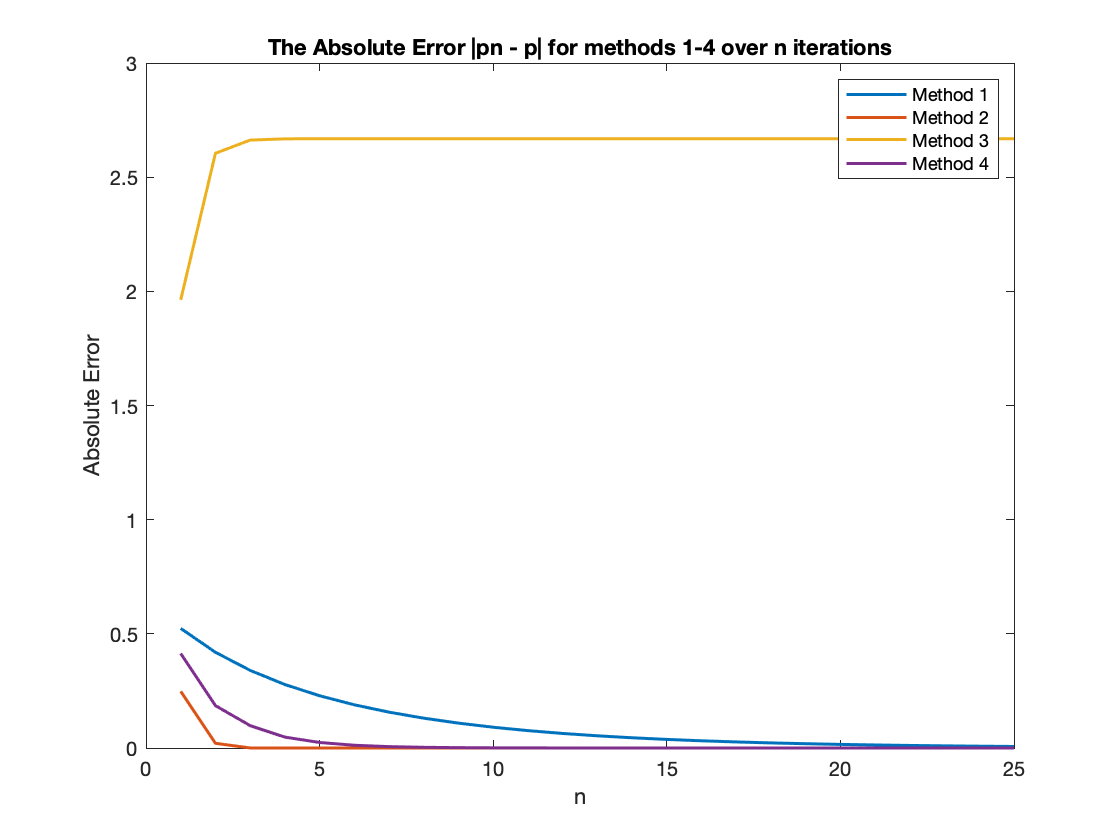
\includegraphics [scale=.25] {Plot_Abs_Error.png}
\end{flushright}
\end{wrapfigure}

Methodology: I used a set number of iterations for all aspects of this project, with $n = 25$.
\flushleft
1. Method 2\\
2. Method 4\\
3. Method 1\\
4. Method 3\\
$~~$\\
Note that method 3 converges second fastest, but is set up as a root finding problem, so it converges to 0, not to the desired solution.\\ 

\section*{Part B}

Methods 1, 2, and 4 are set up as fixed-point problems: they search for where $g(x) = x$. The fewer iterations required for their absolute errors to equal 0, the faster the convergence. From the graph of the absolute errors: method 2 converges fastest, then method 4, then method 1. Method 3 is a root-finding problem of the form $f(x) = g(x) - x = 0$ where $g(x) = x$. For large enough $n$ we have $p_n = 0$, so $|p_n - p| = | 0 - p | = p$. Thus it diverges from our desired solution, but the sequence produced converges to 0, while the absolute error at $n$ converges to $19^{1/3}$ for large enough $n$.

\section*{Part C}

My sincerest thanks to Garrett during workshop hours for assistance with the following process. Let $|p_{n} - p| = e_n$, then $\frac{e_{n+1} }{e_n^\alpha} \approx \lambda \Rightarrow e_{n+1} \approx \lambda e_n ^ \alpha$  for large n. Now consider:

\begin{center}
$e_{n+2} \approx \lambda e_{n+1} ^ \alpha$ \\ 
$~$\\
$\Rightarrow \frac{e_{n+2}}{e_{n+1}} \approx \frac{\lambda e_{n+1} ^ \alpha}{\lambda e_{n} ^ \alpha} = \frac{e_{n+1} ^ \alpha}{e_{n} ^ \alpha}$\\
$~$\\
$\Rightarrow \log \frac{e_n+2}{e_n+1} \approx \log \frac{e_{n+1} ^ \alpha}{e_{n} ^ \alpha} = \alpha( \log e_{n+1} - \log e_n ) = \alpha \log \frac{e_{n+1}}{e_n}$\\
$~$\\
$\Rightarrow \alpha \approx \frac{ log ( \frac {e_{n+2}}{e_{n+1}} )}{ log ( \frac {e_{n+1}}{e_{n}} )}$
\end{center}

By first solving for $\alpha$, I then solved for $\frac{e_{n+1} }{e_n^\alpha} \approx \lambda$, for each method. Note that I used $n = 25$ iterations throughout.

\begin{itemize}

\item Method 1: For $n = 25$, $\alpha \approx  0.9994$, $\lambda \approx 0.8391$. So, this sequence converges to $p$ of order $1$ with asymptotic error constant $\lambda \approx 0.8391 < 1$ and the sequence is said to be linearly convergent.

\item Method 2: For $n = 25$ this sequences converged to $p$, so $\frac{|p_{n+1} - p|}{{|p_n - p|}^\alpha} = \frac{0}{0}$, which is undefined.

\item Method 3: For $n = 25$, $\alpha \approx \frac{ log ( \frac {e_{n+2}}{e_{n+1}} )}{ log ( \frac {e_{n+1}}{e_{n}} ) } = \frac{0}0$, which is undefined.

\item Method 4: For $n = 25$, $\alpha \approx 1$, $\lambda \approx 0.5$. So this sequence converges to $p$ of order $1$ with asymptotic error constant $\lambda \approx 0.5 < 1$ and the sequence is said to be linearly convergent.

\end{itemize}

\end{document}  